
\documentclass[11pt]{article}


\usepackage{graphicx}
\usepackage{amssymb}
\usepackage{hyperref}
\usepackage{fancyvrb}
\usepackage{url}
\usepackage{float}
\usepackage{color}



\title{San Fransisco Crime Classification}
\author{Alison Kingman, James LaManna, Lizzie Kumar}
\date{12/15/2015}

\usepackage{Sweave}
\begin{document}
\Sconcordance{concordance:CrimeDataPaper.tex:CrimeDataPaper.Rnw:%
1 18 1 1 0 38 1 1 28 1 66 22 1 1 2 1 0 1 1 1 2 1 7 5 0 1 3 1 0 1 4 2 0 %
1 1 3 0 1 2 2 1 1 2 1 0 1 2 4 1 1 2 3 0 1 2 10 1 1 6 1 2 1 0 3 1 6 0 1 %
2 2 1 1 2 1 0 2 1 1 6 5 0 2 1 6 0 1 2 11 1}


\maketitle

\section*{Introduction}

For our final project we entered a Kaggle data science competition on San Francisco Crime Classification. The competition's dataset provides nearly 12 years of crime reports from across all of San Francisco. The goal is to predict the category of a crime that occurred, given its time and location. More specifically, the competition requires that we submit a table of probabilities of each category that a crime could possibly be a member of.  The prompt also encourages participants to explore the data set visually as well.	
 
\section*{Importance}

 Predictive policing is a term referring to mathematical methods and data analysis tools developed in the last few years to help law enforcement identify potential criminal activity. This can help police take preventative measures against potential crime or simply decide where to direct their resources. Using these methods has been shown to help police departments save time and money and even cut down crime rates. However, there are serious dangers that come with using historical data for a predictive analysis of crimes. If certain communities in San Francisco are already being overpoliced, the data in its current format will only reflect more crimes in that area. The modeling and exploration we do in this project may be able to give us some information about crime in the city of San Francisco, but we need to be careful about the conclusions we draw from it.

\section*{The Data}

This dataset contains incidents derived from the San Francisco Police Department's Crime Incident Reporting system. The data ranges from 1/1/2003 to 5/13/2015. The training set and test set rotate every week, meaning week 1,3,5,7... belong to the test set, week 2,4,6,8 ... belong to the training set.  Each of the training and test data sets both consist of well over 800,000 crimes. The fields in the given data set are as follows: 
 
 
\begin{itemize}
\item Dates -  timestamp of when the crime occurred
\item Category - Type of crime that was committed. This is the response variable that we are attempting to predict. In total there are 39 different types of crimes in the category data field (train only).
\item Descript - Represents a detailed description of the crime incident (training data only).
\item DayOfWeek  - The day of the week when the crime occurred.
\item PdDistrict -Name of the Police Department District where the crime occurred.
\item Resolution - How the crime incident was resolved (training data only)
\item Address - the approximate street address of the crime incident 
\item X - Longitude
\item Y - Latitude
\end{itemize}

Some initial exploratory charts show that district and location seem to have a relationship with crime frequency and category, which aligns with what we would expect from this type of data.

\begin{center}

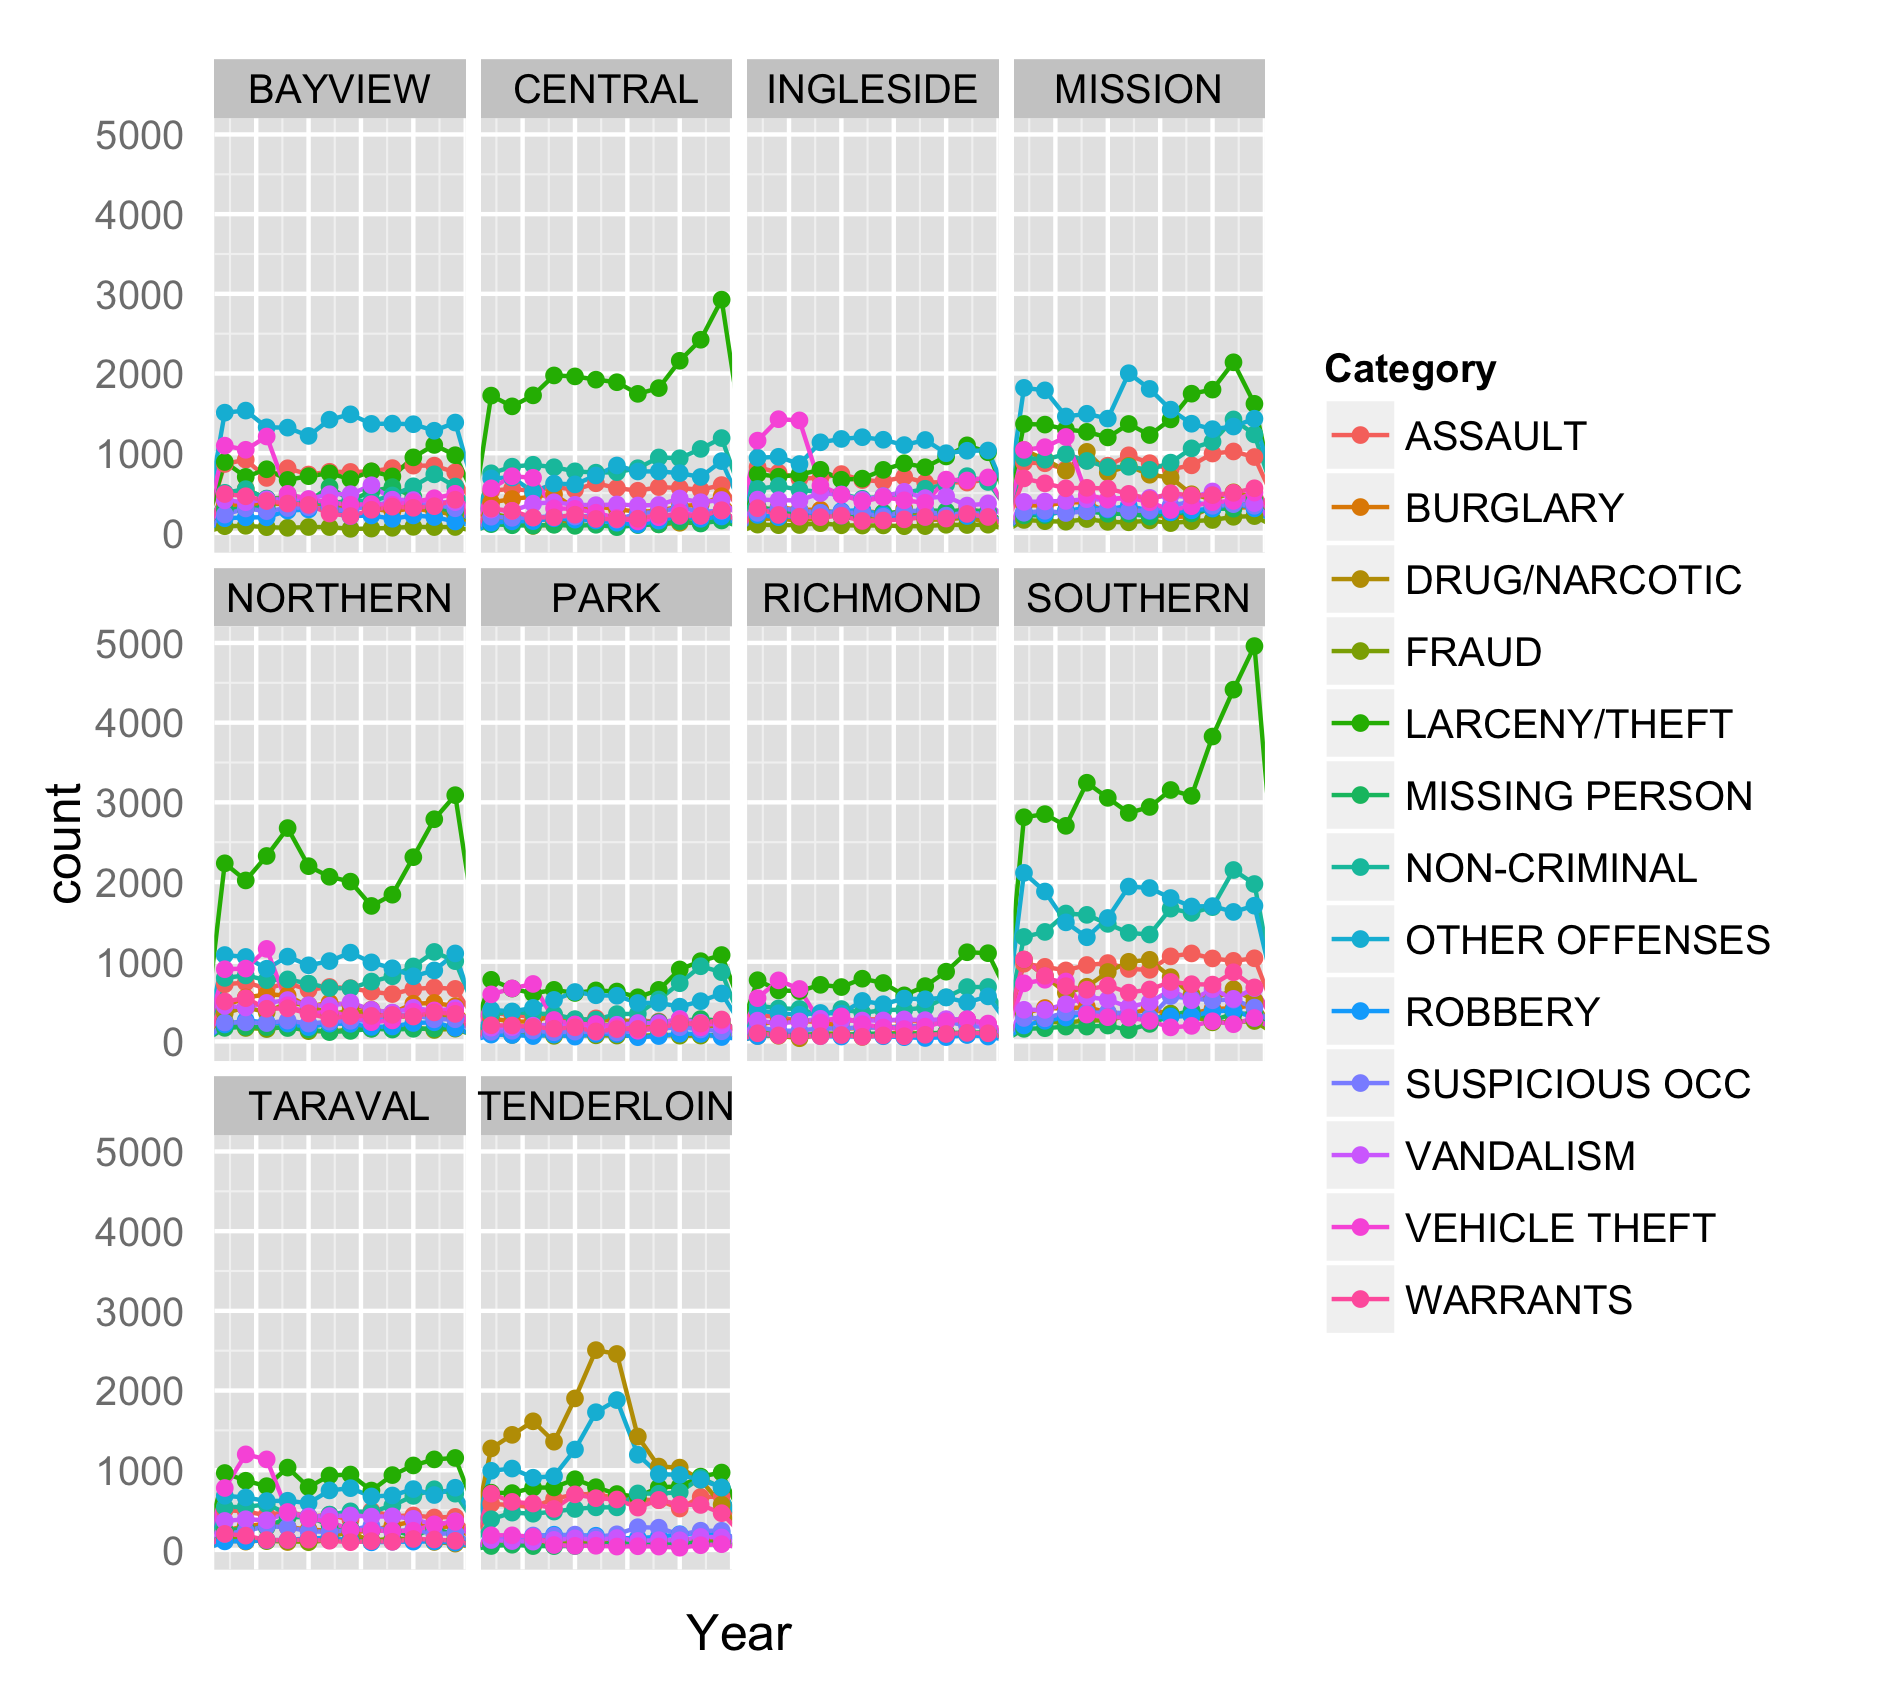
\includegraphics{district-by-cat.png}

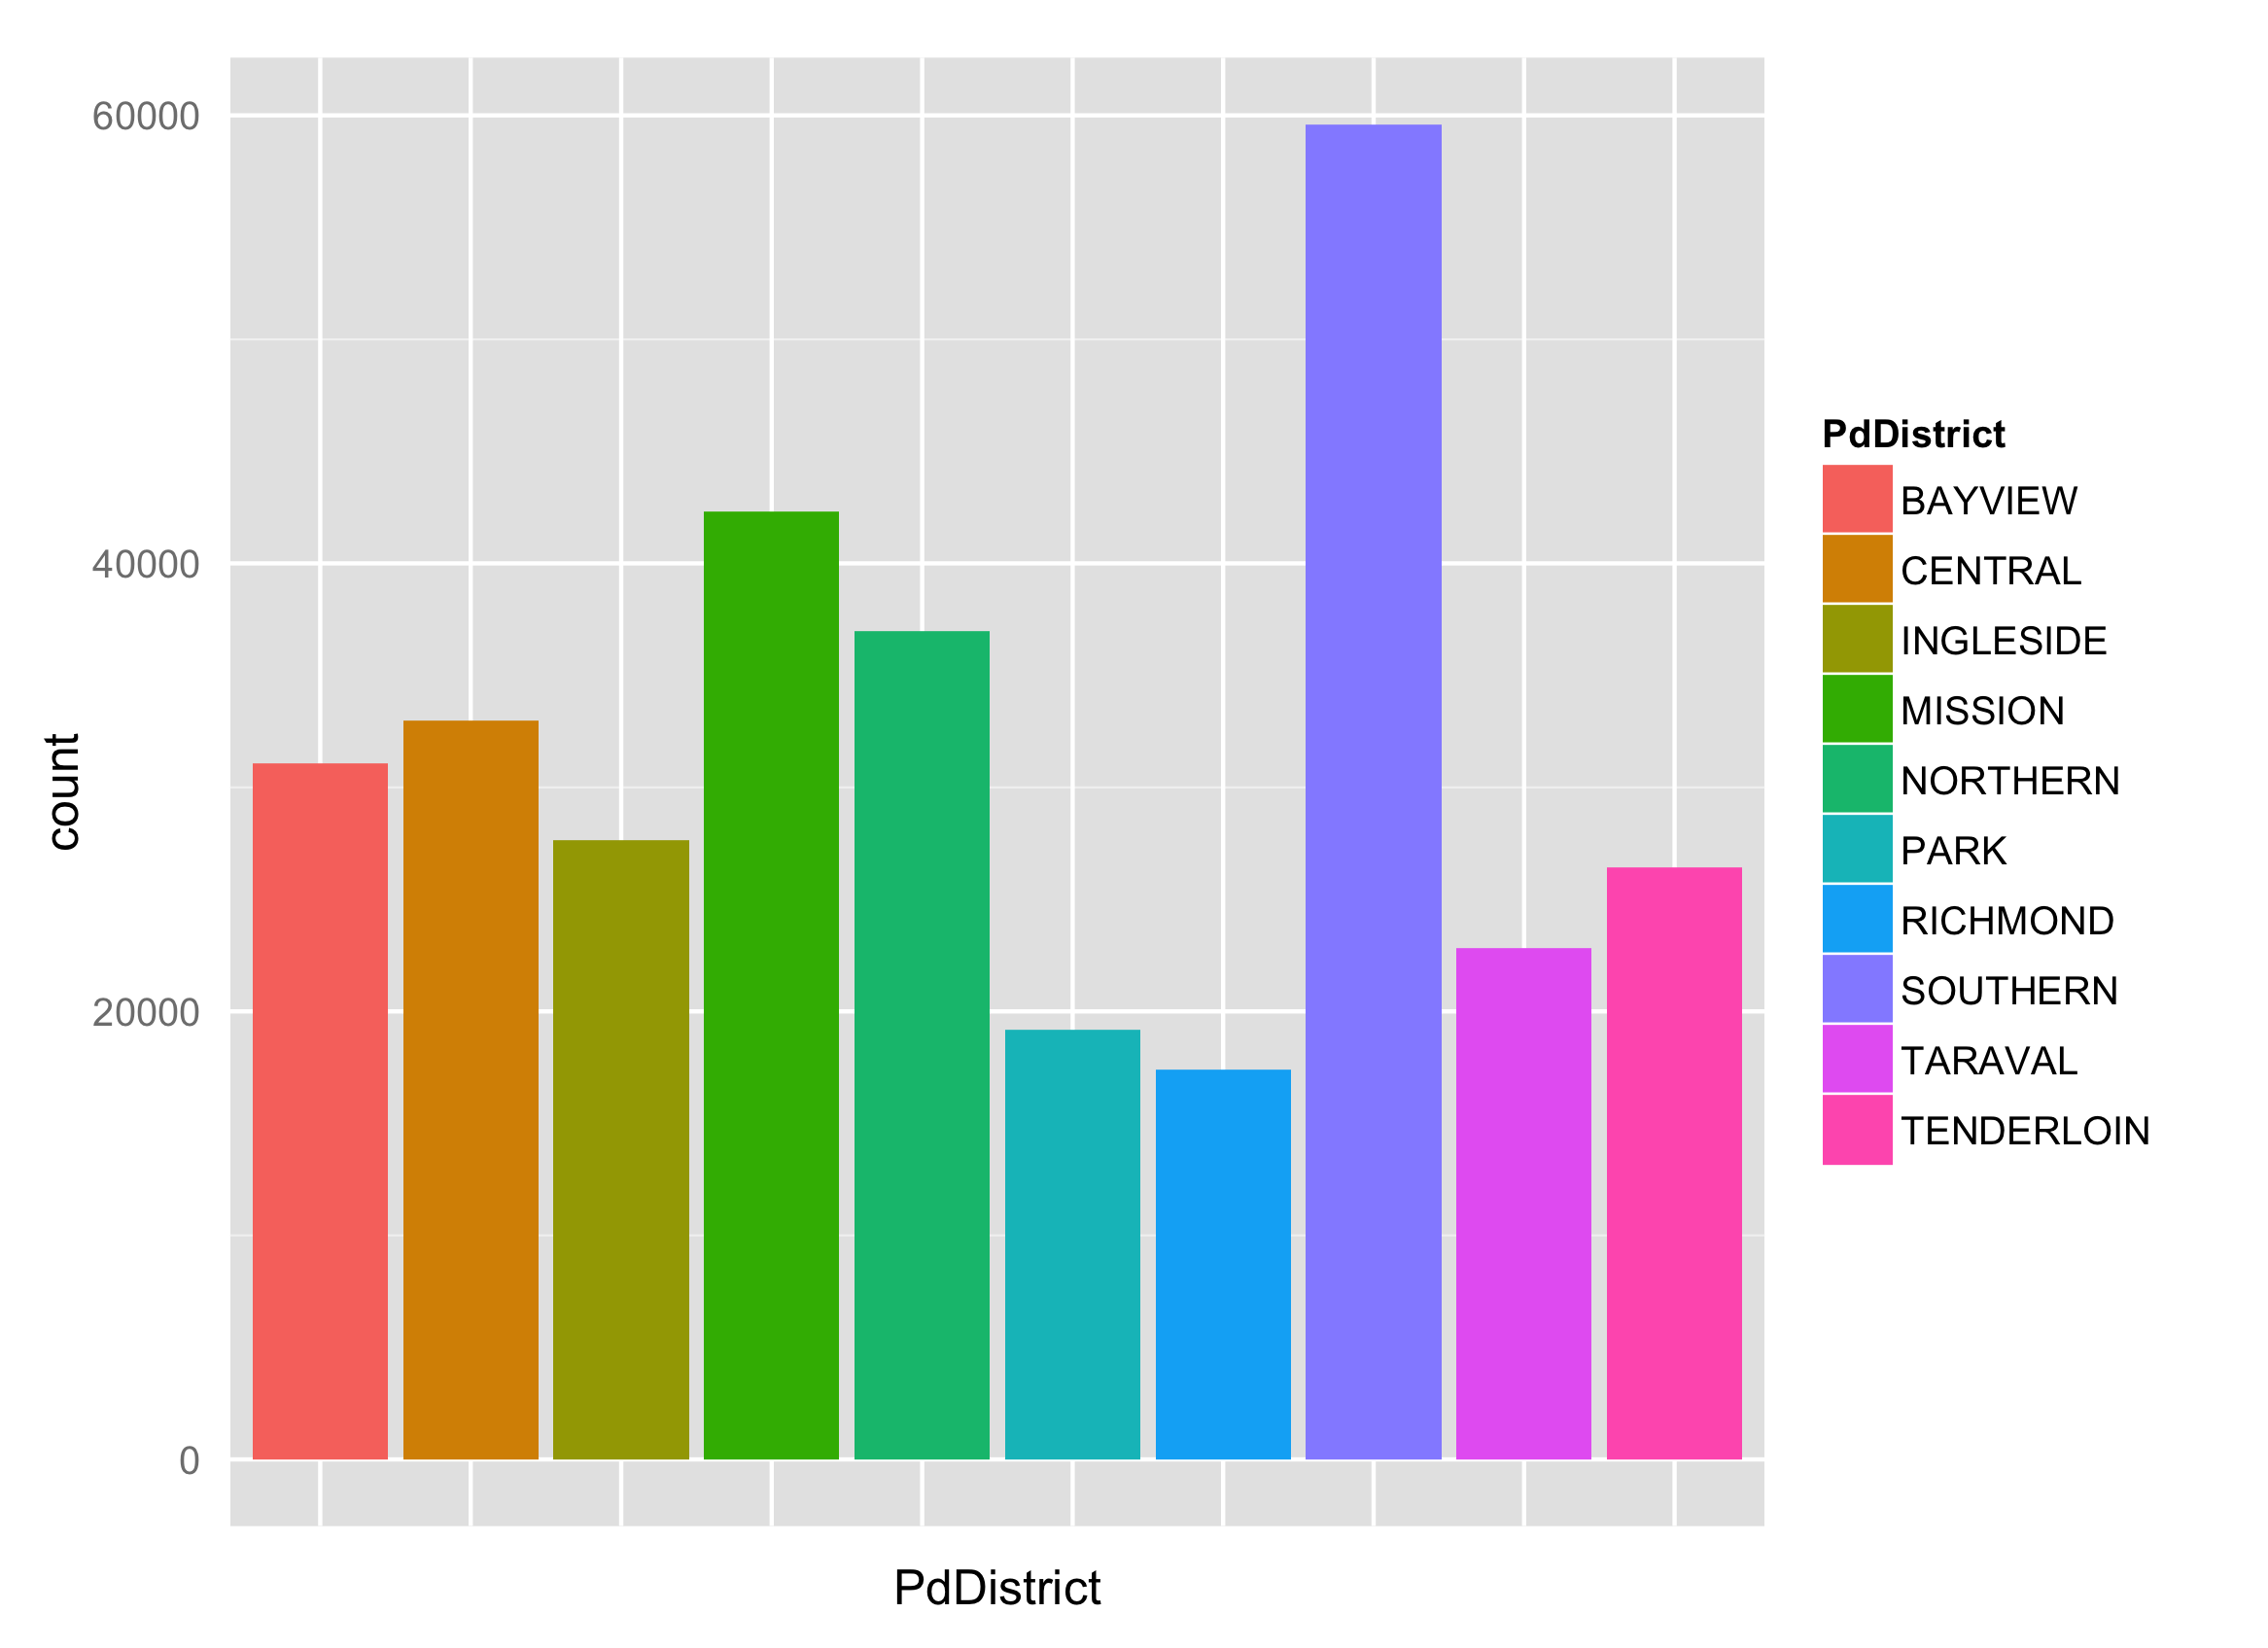
\includegraphics{district-hist.png}

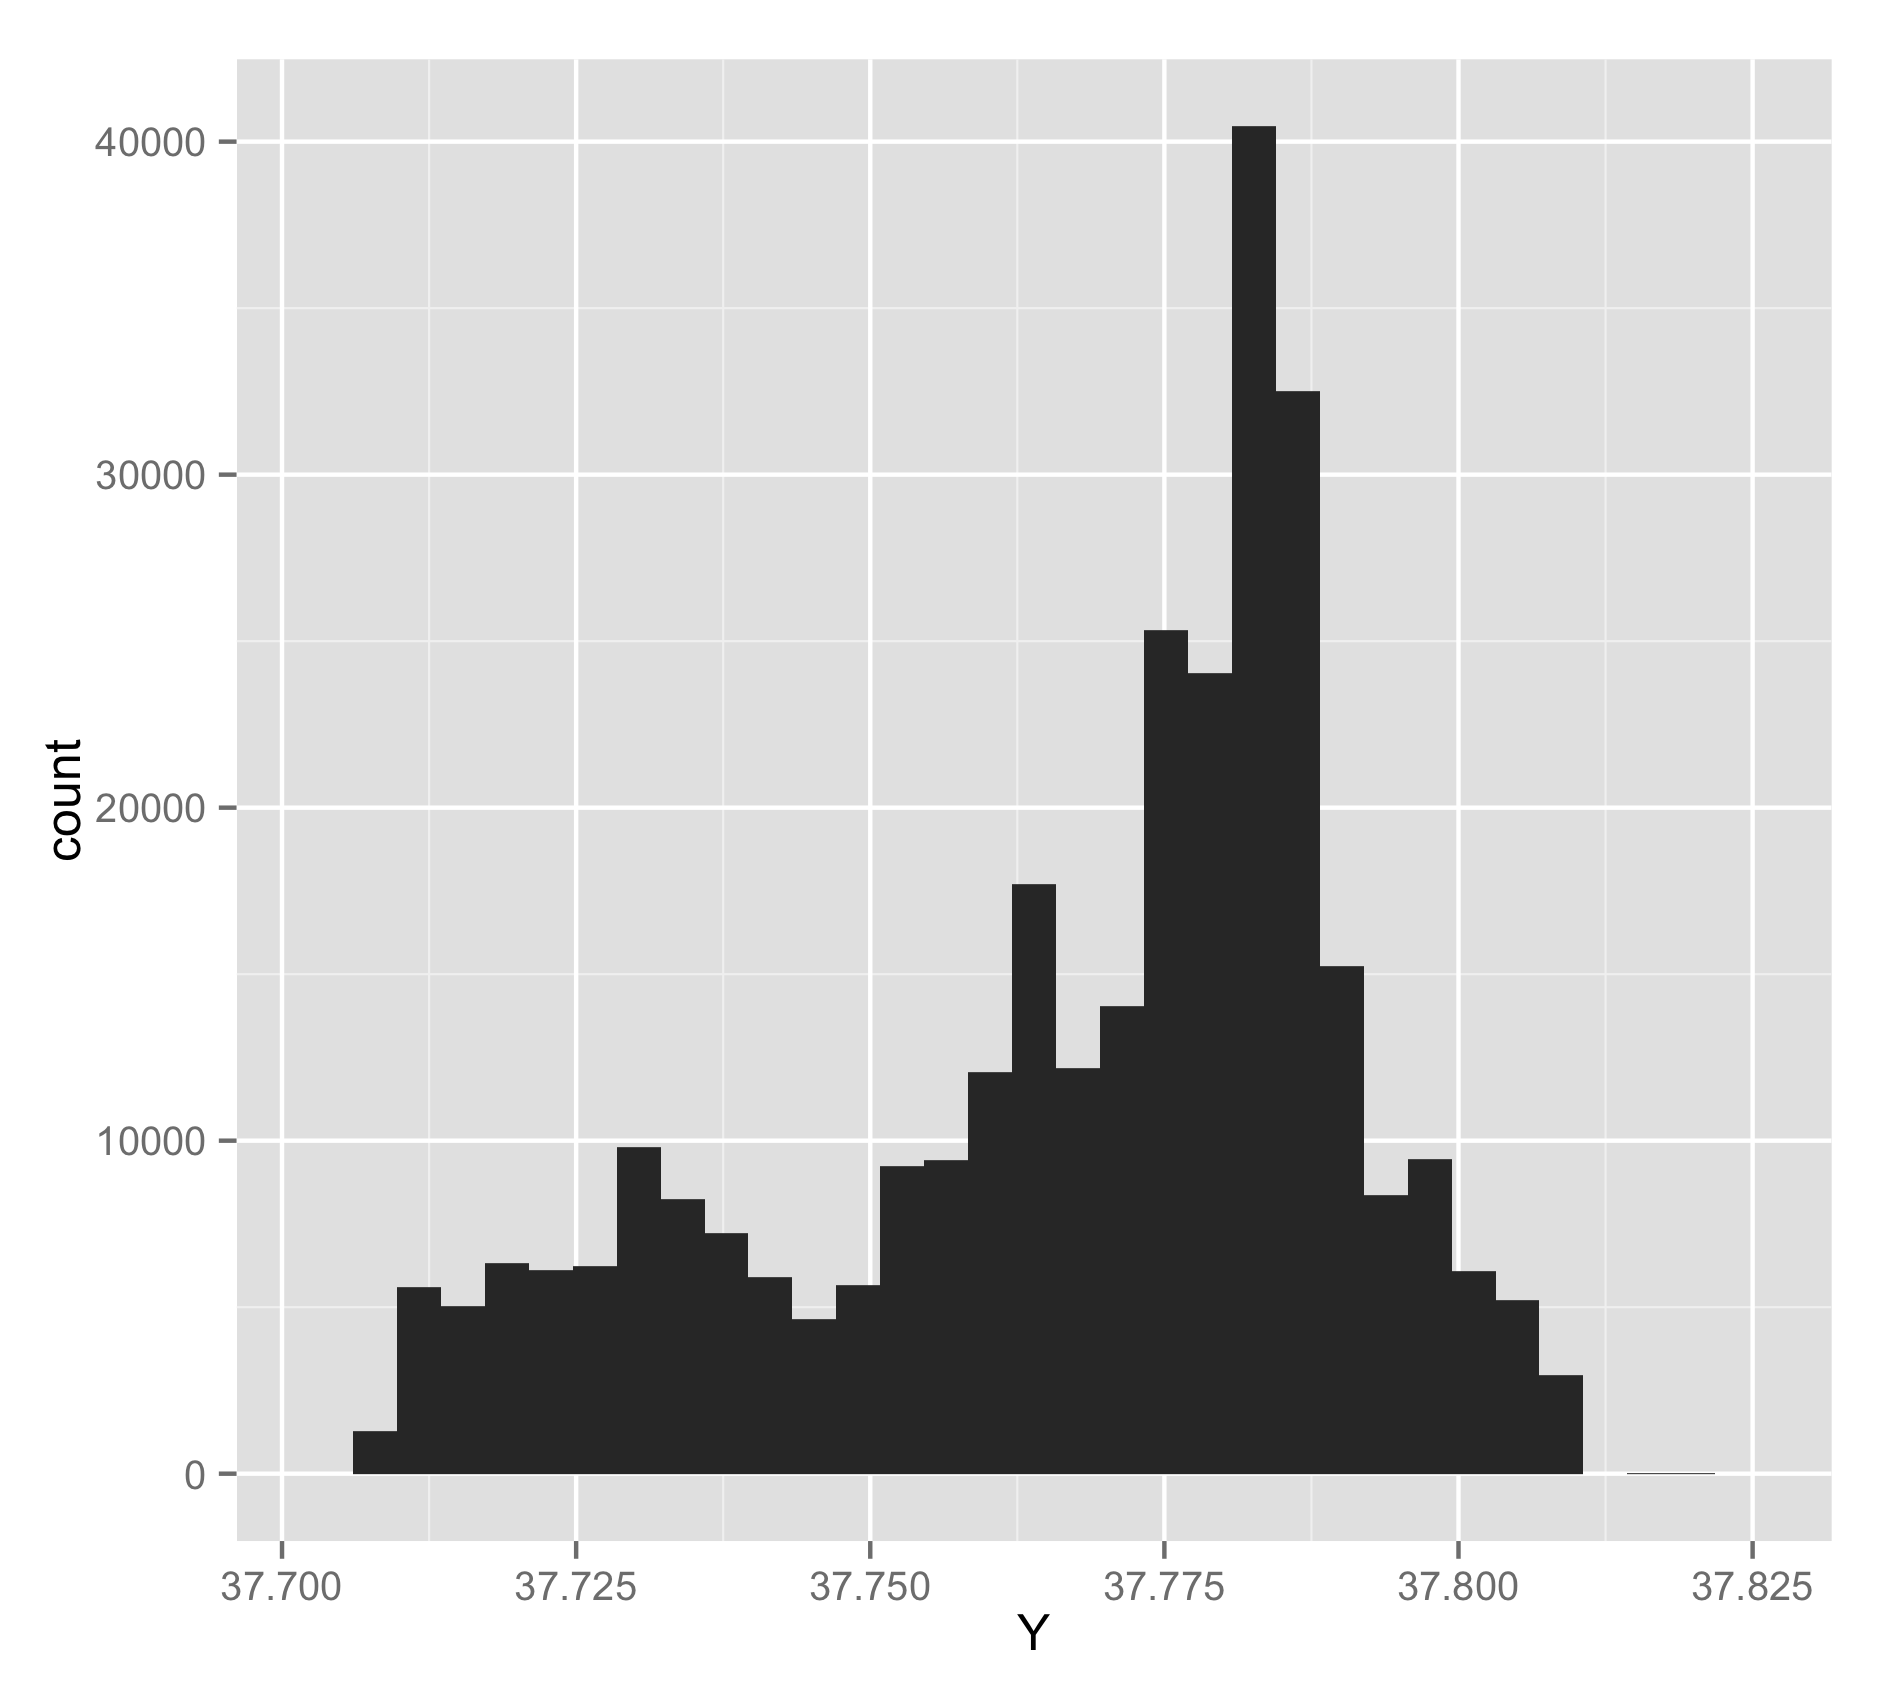
\includegraphics{latitude.png}

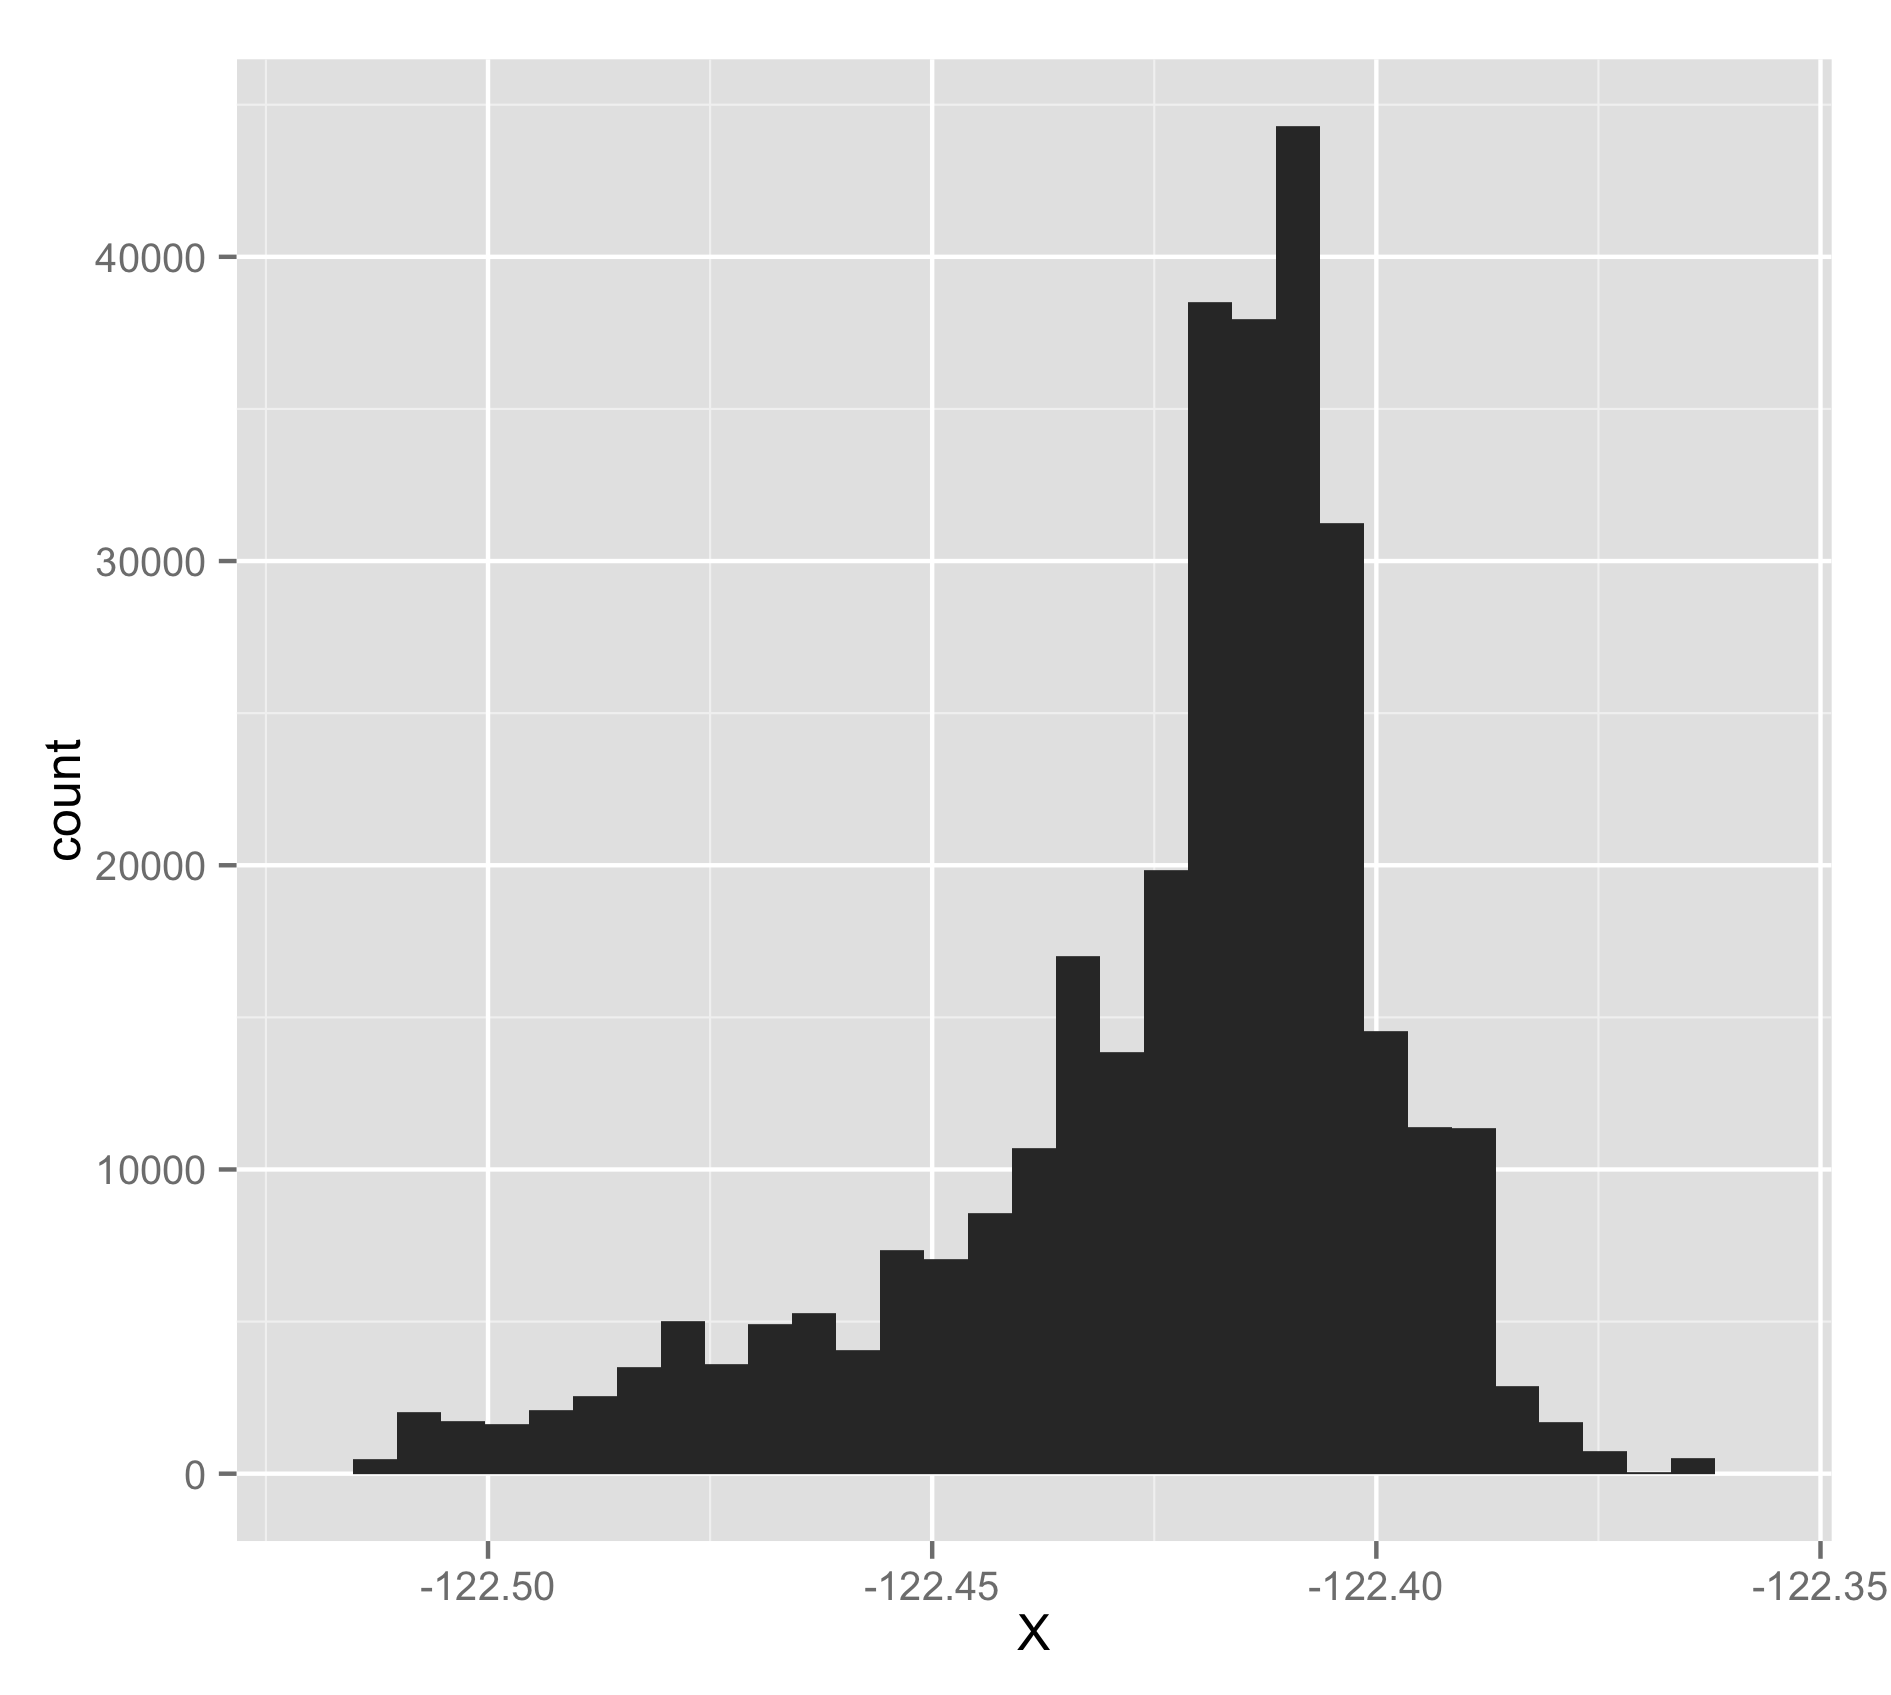
\includegraphics{longitude.png}

\end{center}

A plot of the trends in different crime categories over the last decade reveals nothing particularly troubling other than an sudden drop in vehicle thefts, which was investigated and explained here by another Kaggle user: \url{https://www.kaggle.com/eyecjay/sf-crime/vehicle-thefts-or-jerry-rice-jubilation}

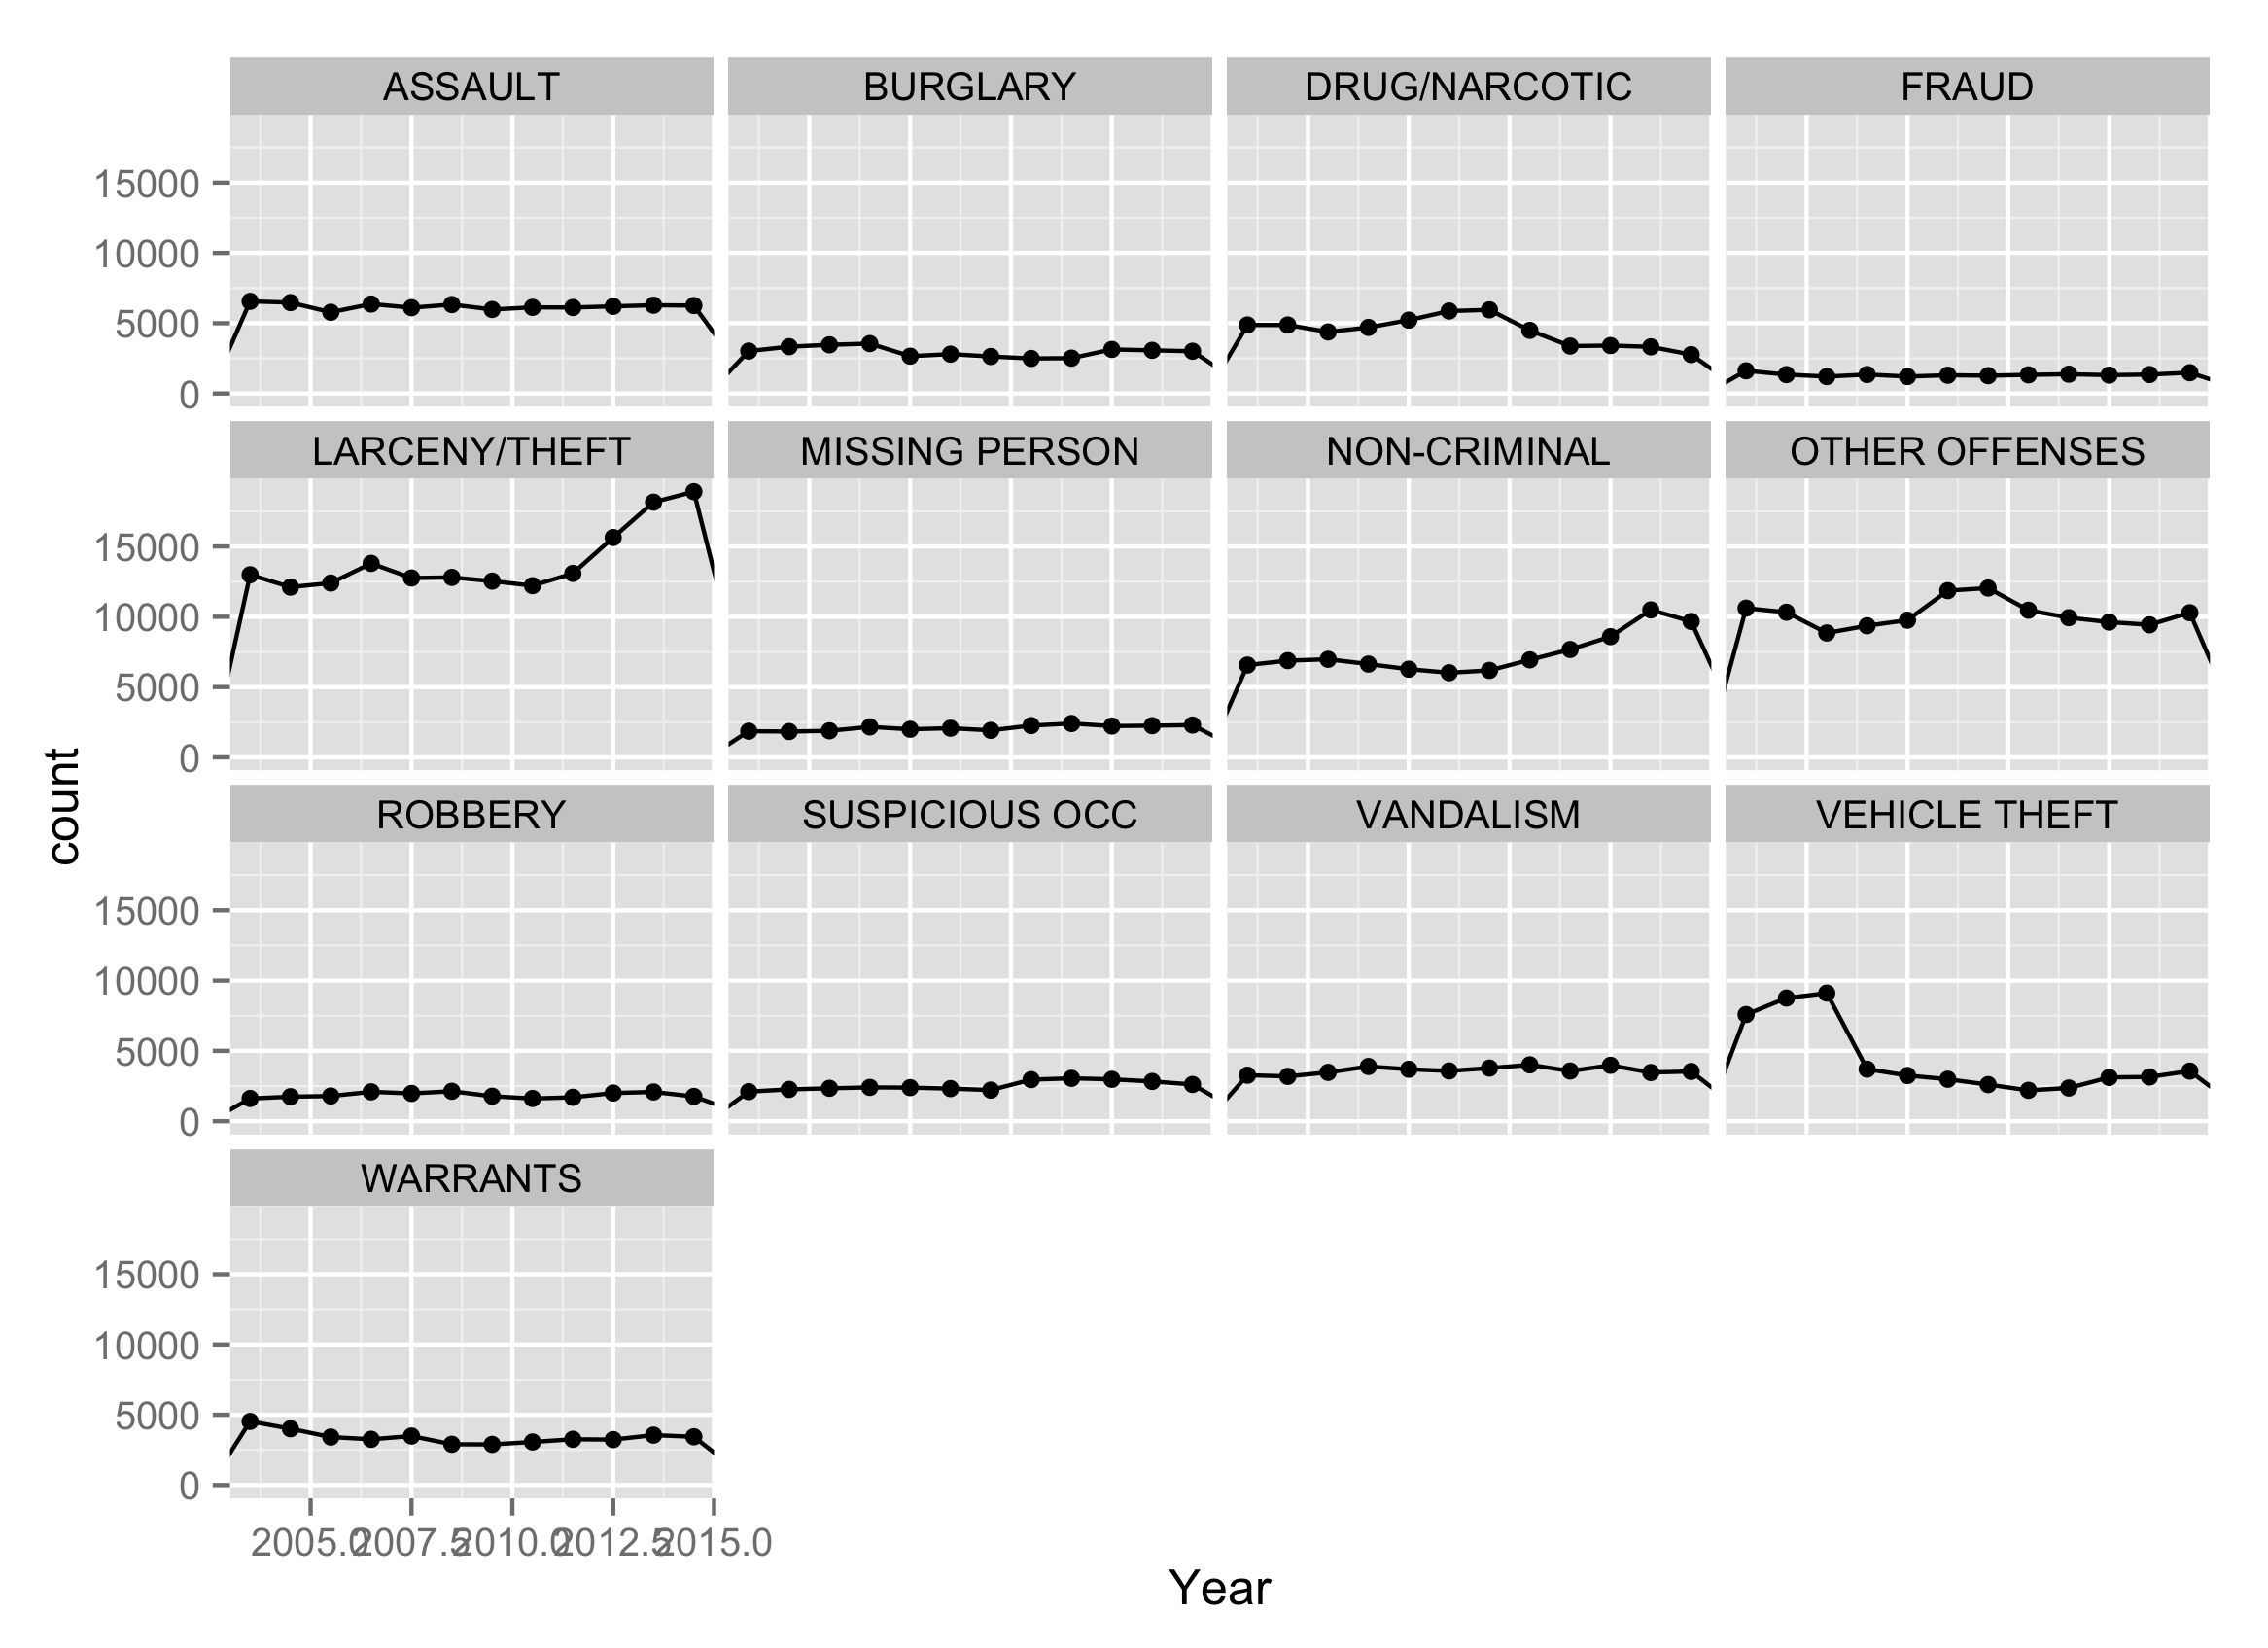
\includegraphics{categories.png}

We were lucky in that our data did not seem to require any wrangling or cleaning to get into a form that we could study and predict.

\section*{Visualization}

To visualize the data we created a shiny application that plots the locations of the top 5 most frequent crimes on a map of San Francisco. In addition, the application has a slider to select a specific year from the data set, and two checkbox groups: one to select the specific type of crime out pf the top five to be displayed and the other is a setting to look at crimes that happened either during the day or night. In addition to the geographic plot of the crime, the Shiny app also includes a bar chart that responds to the same inputs as before but displays the relative frequency of the crimes selected. This bar chart aims to make it easier to compare the amount of occurrences of the types of crimes currently plotted on the map. The visualization can be found via the following url \url{http://rstudio.campus.pomona.edu:3838/jrl31925/CrimeShiny/}
 

The goal of this analysis is to predict the type of crime given a location and time. This shiny app is a nice visualization of the data because it shows the data based on those two criteria. There is a day and night setting as well as a slider for the year component, and the data is plotted on a map of San Francisco, to display the geographic aspect of the data. 



\section*{Method}

We chose a conditional inference tree for the classification of the data.  This classification method work well for this analysis for a few reasons: first, like a standard CART algorithm, this method handles both continuous and categorical variables easily. Second, this model makes it much simpler for us to evaluate the model based on the Kaggle guidelines. Each crime has been labeled with one true class. For each incident, we must submit a set of predicted probabilities (one for every class). The conditional inference tree output includes a set of probabilities for each prediction, thus making it much easier to evaluate our model according to the Kaggle rules. 
 
Conditional inference trees follow the same general algorithm as CART trees. 

\begin{enumerate}
\item Choose variable to split on
\item Find best split point to partition on.
\item Repeat for the two partitions. Stop on stopping condition. 
\end{enumerate}

In CART trees, the variable splitting can be done by optimizing some parameter, such as the Gini index. In conditional inference trees however, we choose the variable to split on by using conditional inference through permutation test.

To determine the best variable to split on, we choose the null hypothesis  $H_0 = \cap_{j=1}^{m}  H_0^j : P(Y|X_j) = P(Y)$ where $Y$ is the response variable and the $X_j’s$ are the explanatory variable. That is, the null hypothesis is that the probability of making a prediction given an explanatory variable is exactly the same as making that prediction without any knowledge of the explanatory variable.  Through a permutation test, we can calculate p-values for each of the explanatory variables. If all p-values are chosen above a certain threshold (for example, 0.05), then we do not reject the null hypothesis and we terminate the node.  If  we reject the null hypothesis, we choose the explanatory variable with the lowest p-value to split on. 
 

 
\section*{Implementation}

Before running the model, we first needed to modify  our explanatory variables. We extracted the hour, month and year and made them factor variables. We also removed all data before 2005 because the amount of vehicle thefts, suddenly dropped after this year. This unnatural drop off in occurrences was likely to due a reporting change or some other outside factor.  Finally, we filtered out unneeded columns such as resolution and description. In our analysis, we included hour, month, year and district as categorical variables and latitude and longitude as continuous variables. 

\begin{Schunk}
\begin{Sinput}
> require(lubridate)
> require(dplyr)
> data= read.csv("../../train.csv")
> #Extract  hour, month and year from timestamp
> data = data %>% 
+   mutate(Time = ymd_hms(Dates)) %>%
+   mutate(hour = as.factor(hour(Time)), 
+          month = as.factor(month(Time)), 
+          year=year(Time))
> #remove description, resolution address and date columns
> data = data[,-c(1,3,6,7,10)]
> #remove data before recorded before 2006
> data = data %>%
+   filter(year >2005)
> data$year = as.factor(data$year)
\end{Sinput}
\end{Schunk}

The Conditional Inference Tree model is computationally intense. Since our data has about 800,000 observations and 39 categories of crime, training the conditional inference tree with it takes a long time. Therefore, we made a few more modifications to cut down on our run time. We choose to keep all of the categories that had more than 10,000 representations in the training data and classified everything else as other, giving us a total of 13 categories. We decided to train the model on 50,000 randomly sampled observations from the training data, which took approximately 1.2 days. 

\begin{Schunk}
\begin{Sinput}
> require(partykit)
> set.seed(100)
> trainsize = 50000
> trainind = sample(seq(1:nrow(data)), trainsize)
> train= data[trainind,]
> test = data[-trainind,]
> t = ctree(Category~., data = train)
\end{Sinput}
\end{Schunk}
  
\section*{Results}

When implementing the model, we modified the categories of the training data. We tested the remaining data twice: once with the modified 13 categories and once with the original 39 categories. Note that in both cases, we used the same training set.  We present the results for each in the form of a test error and logloss calculation. The log loss is defined as 

\[ logloss = - \frac{1}{N} \sum_{i=1}^N \sum_{j=1}^M y_{ij} \log (p_{ij}) \]

$N$ is the total number of observations and $M$ is the total number of categories. $y_{ij} = 1$ if  observation $i$ is in category $j$ and 0 otherwise. $p_{ij}$ is the predicted probability that observation $i$ is in category $j$. The logloss is the score that Kaggle teams compete to minimize.

First, we examine the results of test data with the modified categories. The test error is 70.6\%. This error rate is higher than we would like .


\begin{Schunk}
\begin{Sinput}
> pred = predict(t, test)
> tab = table(pred, test$Category)
> error = (nrow(test) - sum(diag(tab)))/nrow(test)
> error
\end{Sinput}
\begin{Soutput}
[1] 0.7059887
\end{Soutput}
\end{Schunk}

Next, we find the logloss of the test  data. to be 2.31. On the  Kaggle  leaderboard, the logloss scores between 2 and 34 with low scores being preferable. About 5.7\% of the teams have a score less than 2.31. 

\begin{Schunk}
\begin{Sinput}
> probpred = predict(t, test, type="prob")
> N = nrow(test)
> logprobs = rep(1,N)
> for (i in seq(1,N)){
+   class = test$Category[i]
+   prob = probpred[i, class]
+   prob = max(min(prob,1-10^(-15)), 10^(-15))
+   logprobs[i] = log(prob)
+ }
> logloss = -sum(logprobs)/N
> logloss
\end{Sinput}
\begin{Soutput}
[1] 2.316695
\end{Soutput}
\end{Schunk}

We repeat the calculation above for the test data with the original categories. The test error is 97.4\% and the logloss is 10.4. About 79.3\% of the teams on the kaggle leaderboard have a score lower than 10.4

\section*{Limitations and Conclusions}

In our results, we have very poor test error rates. We examine possible reasons for this. First, if we examine the visualizations of the data from the shiny application, we see that most of the crimes tend to occur in the same area of Northeast San Francisco. Also, when we visualize the data by the time of day, there also does not seem to be a  significant difference between daytime and nighttime crimes. Since the explanatory variables for all observations are so similar, the conditional inference tree is not able to accurately classify a crime to one of the many categories. Another issue is that training a conditional inference tree is very computationally intensive. It took 1.2 days to train on 50,000 data points which is only about 6\% of the given training data. It is possible that the tree might not have been able to accurately build the tree since most of the observations have been left out. However, when we build the tree using 1000, 10,000 and 50,000 observations, the errors did not seem to improve when increasing the training size. Therefore, the cause for our poor errors is most likely due to the similarity of the explanatory variables across categories rather than our inability to train with the full data set. 

Overall, a conditional inference tree probably was not the best model for this data. The data had too many observations and too many classification categories. A data set with fewer observations and classification categories might have better results. 



\end{document}
